\documentclass[a4paper]{article}

\usepackage[sort]{natbib}
\usepackage{fancyhdr}


% \documentclass[a4paper]{article}

\usepackage[english]{babel}
\usepackage[utf8]{inputenc}
\usepackage{amsmath}
\usepackage{graphicx}
\usepackage[colorinlistoftodos]{todonotes}
\usepackage{hyperref}
\usepackage{booktabs} % To thicken table lines
\usepackage{tablefootnote}
\usepackage{listings}
% \usepackage[numbers]{natbib}

\usepackage{graphicx}
\usepackage{babel,blindtext}

\usepackage{algorithm}
\usepackage[noend]{algpseudocode}


% Uirá packages
\usepackage{algorithm}
\usepackage[noend]{algpseudocode}
\usepackage{booktabs} % To thicken table lines
\usepackage{graphicx}
\usepackage{babel,blindtext}
\usepackage{amsmath}
\usepackage[colorinlistoftodos]{todonotes}
\usepackage{hyperref}
\usepackage{mathtools}
\usepackage{listings}
\usepackage{epstopdf}



% you may include other packages here (next line)
\usepackage{enumitem}



%----- you must not change this -----------------
\oddsidemargin 0.2cm
\topmargin -1.0cm
\textheight 24.0cm
\textwidth 15.25cm
% \parindent=0pt
\parskip 1ex
\renewcommand{\baselinestretch}{1.1}
\pagestyle{fancy}
%----------------------------------------------------



% enter your details here----------------------------------

\lhead{\normalsize \textrm{Collaboration and Competition}}
\chead{}
\rhead{\normalsize November 08, 2018}
\lfoot{\normalsize \textrm{DRLND - Udacity}}
\cfoot{}
\rfoot{Uirá Caiado}
\setlength{\fboxrule}{4pt}\setlength{\fboxsep}{2ex}
\renewcommand{\headrulewidth}{0.4pt}
\renewcommand{\footrulewidth}{0.4pt}


\begin{document}


%----------------your title below -----------------------------

\begin{center}

{\bf \large { Learning to Collaborate With Deep Reinforcement Learning \\ \small Uirá Caiado}}
\end{center}


%---------------- start of document body------------------

% The report clearly describes the learning algorithm, along with the chosen hyperparameters. It also describes the model architectures for any neural networks.

According to \cite{NIPS2017_7217}, many important applications involve interaction between multiple agents, as multi-robot control,  analysis of social dilemmas and so on. However, multi-agent environments present additional challenges for traditional reinforcement learning (RL) approaches. As each agent's policy is continually changing, the environment becomes non-stationary from the perspective of any
individual agent.

 In this project, I used the Multi-Agent Deep Deterministic Policy Gradient (DDPG) model to solve the Unity Tennis\footnote{Source: \url{https://bit.ly/2OOkxKo}} environment, where two agents control rackets to bounce a ball over a net. A reward of +0.1 is provided for each step that the the agent hits the ball over the net. If the agent lets a ball hit the ground or hits the ball out of bounds, it receives a reward of -0.01.
 
 The observation space consists of 8 variables corresponding to the position and velocity of the ball and racket. Each agent receives its own, local observation.  Two continuous actions are available, corresponding to movement toward (or away from) the net, and jumping. To solve the environment, the agents must get an average score of +0.5 (over 100 consecutive episodes, after taking the maximum over both agents).

% describes the model architectures for any neural networks

The algorithm implemented in this project uses an actor-critic architecture to deal with the high-dimensional action space. As described by \cite{Lillicrap:2015ww}, the model maintains a parameterized actor function $\mu(s | \theta^{\mu})$ which specifies the current policy by mapping states to a specific action. The critic $Q(s, a; \;\theta)$ is learned using the Bellman equation as in Q-learning and is used to evaluate the actions chosen by the actor. The resulting evaluation is used to compose a baseline (or advantage function) that is then used to train the actor model. 
 
 The parameters $\theta$ from both actor and critic models are learned by neural networks with almost the same architecture. The input to these networks consists of a matrix $24 \times 1$ produced by the environment and the first layer is a fully-connected linear layer with $400$ neurons and applies a rectifier nonlinearity. It is followed by a hidden layer also consisting of a fully-connected linear layer with $300$ neurons followed by another rectifier. The output layer of the actor-network consists of a fully-connected linear layer with a vector $2\times1$ as output for each agent. The output layer of the critic network includes a fully-connected linear layer with a single output for each agent followed by a \textit{tanh} activation function that naturally constrains the values between $[-1, 1]$. For the model used in this project, the critic network have some particularities. First, the actions are included in the first layer of the critic network, similar to what was done by \cite{Lillicrap:2015ww}. Second, as proposed by  \cite{NIPS2017_7217}, the critic network is augmented with extra information about the state and actions of the other agent, so the input space size is doubled.

% (1) describes the learning algorithm, along with the chosen hyperparameters
The MADDPG model was introduced by \cite{NIPS2017_7217}, and it is an extension of the DDPG algorithm, proposed by \cite{Lillicrap:2015ww}. One of the main differences from the original model is that, while the critic is trained with extra information about the policies of other agents, as explained before, the actor only has access to local information.

The role of the actor in this method is to estimate the stochastic policy that returns the probability distribution over the actions. The critic is used to calculate the Q-values of the actions so it can be updated using the Bellman equation to find the approximation of $Q(s, a)$ and minimizing the MSE objective. As explained by \cite{Lillicrap:2015ww}, the actor is updated by applying the chain rule to the expected return obtained by the critic network from the actor parameters. As this method is off-policy, we can use the same tricks used by the DQN model, presented by \cite{mnih2015humanlevel}, as the replay buffer and the use of local/target networks to help stabilize the parameters of both actor and critic.

I used a replay buffer size of $100,000$ experiences, mini-batches of $200$ instances and a $\gamma=0.99$ to discount the rewards. The learning rate of the actor was $0.0001$, to the critic was $0.001$, and the networks were updated every two steps. As suggested by \cite{Lillicrap:2015ww}, the target networks slowly tracked the local networks using $\tau=0.001$. For detail on how each one of these parameters was used in the model, check the papers cited or the code provided along with this report.

 % The submission reports the number of episodes needed to solve the environment.

Different from the original paper, I used a separated actor and critic networks for both agents. Also, both local and target networks presented the same architecture, described before. Using this configuration, I was able to solve the environment in $1764$ episodes. The figure \ref{fig:ddpg} presents the results of the simulation. The left panel exposes the rewards obtained in each episode and, in the right panel, I plotted a moving average of the last $100$ episodes of this rewards. The shaded area corresponds to one standard deviation $\sigma$ of the rewards of those $100$ episodes.

% A plot of rewards per episode is included to illustrate that the agents get an average score of +0.5 (over 100 consecutive episodes, after taking the maximum over both agents).
\begin{figure}[ht]
\centering
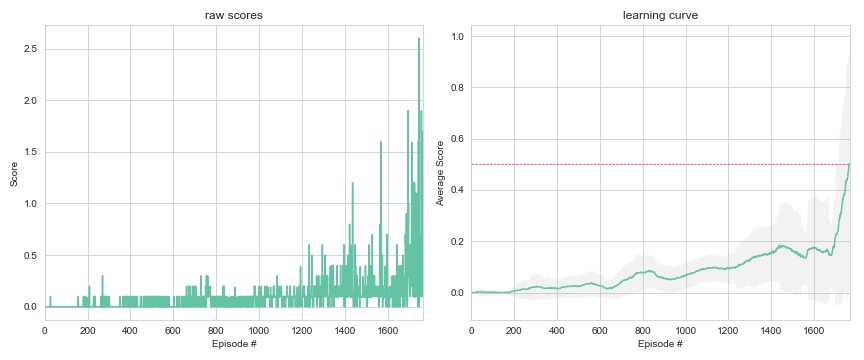
\includegraphics[width=0.65\textwidth]{../notebooks/figures/2018-11-07-MADDPG-learning-curve.jpg}
\caption{MADDPG - Learning Curve(left panel) and Moving-average(right panel)}
\label{fig:ddpg}
\end{figure}

% The submission has concrete future ideas for improving the agent's performance.
Finally, as some possibles extensions, the parameters of the models could be better tuned, and another model could be added to the analysis, as the Proximal Policy Optimization (PPO) method, introduced by \cite{Schulman:2017vq}. We could use the policy network as the actor-network and include an augmented critic network, as in MADDPG,  to deal with the action continuous space and the multiagent environment.




% ----------------end of document body---------------------

%---------------- start of references------------------

\bibliographystyle{plain}
% or try abbrvnat or unsrtnat
\bibliography{biblio.bib}

%---------------- end of references------------------


\end{document}
